\documentclass[journal, dvipsnames]{IEEEtran}
\usepackage{orcidlink}
\usepackage{array}
\usepackage{ducksay}
% \usepackage{polyglossia}
\usepackage[english]{babel}
\usepackage{fontspec}
% \usepackage{unicode-math}
% \usepackage{minted}

% \setmonofont{JuliaMono-Bold.ttf}[
%     Contextuals = Alternate,
%     CharacterVariant=1,
%     Scale = MatchLowercase,
%     BoldFont = JuliaMono-Bold.ttf,
%     Numbers = OldStyle
% ]

\usepackage[caption=false,font=normalsize,labelfont=sf,textfont=sf]{subfig}
%% Useful packages
% https://www.overleaf.com/learn/latex/Typesetting_quotations#csquotes_package
\usepackage{csquotes}
% for svg https://tex.stackexchange.com/questions/442077/is-it-possible-to-use-svg-images-with-overleaf
\usepackage{svg}
\usepackage{tikzbricks}
\usepackage{tikzducks}
% For table
\usepackage{colortbl}


% For references
\usepackage[backend=biber, style=numeric]{biblatex}
\addbibresource{fedLearning.bib} % Replace with your actual BibTeX file
\addbibresource{principles.bib}
\addbibresource{OGHPapers.bib}
\addbibresource{KMS.bib}
\addbibresource{gbif.bib}
% For referring to description items
% use like
% \begin{description}
%     \descitem{item name}{itLabel}
% \end{description}
% \descref{itLabel} $\rightarrow$ [item name](the_item)
% https://tex.stackexchange.com/a/293/241038
\newcounter{desccount}
\newcommand{\descitem}[2]{
  \item[#1] \refstepcounter{desccount}\label{#2}%
  \expandafter\xdef\csname#2\endcsname{#1}%
}

\newcommand{\descref}[1]{\hyperref[#1]{\csname#1\endcsname}}


% For flowchart
\usepackage{tikz}
\usetikzlibrary{shapes.geometric, arrows}
\tikzstyle{startstop} = [rectangle, rounded corners, minimum width=2cm, minimum height=1cm,text centered, text width=2cm, draw=black, fill=red!30]
\tikzstyle{io} = [trapezium, trapezium left angle=70, trapezium right angle=110, minimum width=2cm, minimum height=1cm, text centered, text width=2cm, draw=black, fill=blue!30]
\tikzstyle{process} = [rectangle, minimum width=2cm, minimum height=1cm, text centered, text width=2cm, draw=black, fill=orange!30]
\tikzstyle{decision} = [diamond, minimum width=2cm, minimum height=1cm, text centered, text width=2cm, draw=black, fill=green!30]
\tikzstyle{arrow} = [thick,->,>=stealth]


% correct bad hyphenation here
\hyphenation{op-tical net-works semi-conduc-tor}
\hypersetup{colorlinks=true}

\title{Creating a Visual Framework and Implementation for FAIR-TRUST-CARE Compliant Data Sharing Repositories under GDPR Legislation}
\author{Fee Gevaert \orcidlink{https://orcid.org/0009-0008-2311-6336} \today{}}

\begin{document}

\maketitle

\begin{abstract}
A visual overview system of FAIR-TRUST-CARE, GEOSS principles and GDPR legislation is presented that allows embedding it into various computer architecture designs. Different computer architecture designs and options are laid out that allow the reader to mix-and-match a solution that adheres to the principles. Lastly, a specific implementation is described in Nextcloud for secure data sharing. This work aims to provide a versatile framework for incorporating essential principles into computer architecture designs.
\end{abstract}

\section{Introduction}
\IEEEPARstart{M}{y} internship project, titled "Implementing and evaluating digital infrastructure for consensual data sharing to empower data holders in bottom-up governance of environmental outcomes," is a pioneering response to a multi-disciplinary challenge that is both intricate and dynamic. The core of this challenge resides at the crossroads of diverse domains: legal mandates, such as the General Data Protection Regulation (GDPR); societal values encapsulated in the CARE principles \cite{carrollCAREPrinciplesIndigenous2020}; the technical underpinnings of FAIR data \cite{jacobsenFAIRPrinciplesInterpretations2020, wilkinsonFAIRGuidingPrinciples2016, lamprechtFAIRPrinciplesResearch2020}; and the amalgamation of technical and governance ideals embodied in TRUST \cite{linTRUSTPrinciplesDigital2020}, as well as considerations that went into designing the GEOSS architecture \cite{christianGEOSSArchitecturePrinciples2008}. This intricate web of influences underscores the complexity of the task at hand.

Specifically, OpenGeoHub (OGH) processes petabyte-scale data using Machine Learning \cite{bouasriaPredictivePerformanceMachine2023a} to generate an array of predictive maps, covering erosivity \cite{panagosGlobalRainfallErosivity2023}, soil properties \cite{henglSoilGrids250mGlobalGridded2017}, carbon sequestration \cite{maxwellGlobalMangroveSoil2023}, biome changes under climate change \cite{bonannellaBiomesWorldClimate2023}, and more \cite{hacklanderLandPotentialAssessment2023}. An integral component of these machine learning models is the utilization of in-situ data, which is considered sensitive within the project (WP7.2) and thus falls under GDPR legislation. This scenario exemplifies the central contradiction we aim to address: the imperative for data to be as open as possible, juxtaposed with the need for stringent controls on storage, processing, and sharing of sensitive data.

This contradiction becomes even more pronounced when viewed through the lens of the CARE principles, which uphold the rights of indigenous peoples to access their own data while retaining the authority to govern who gathers, accesses, and processes this data. Our mission is to navigate this intricate terrain, crafting a digital infrastructure that not only adheres to these principles but also empowers data holders to participate actively in the governance of environmental outcomes. Through this project, we embark on a journey that transcends legal, ethical, technological, and governance boundaries, striving to create a harmonious and open environment for data sharing and informed decision-making.

The addressed knowledge gap in this report is that there is no clear overview of design principles and no implementation of a data sharing platform that adheres to all of these principles. Additionally, within OGH, there was no clear overview of different Free and Open Source Softwares (FOSS) with which such a system could be implemented. This document aims to be a high level overview as well as a start for alternative implementations. As a high-level overview, it explains considerations that went into the current development of the plugin. As a start for further development, it links to relevant information and code.

In writing this report, effort has been made to make the overview understandable to non-technical readers, while providing links to more in-depth sources. In this way, it could also be used as a start to build on top of the progress made during my internship. Where relevant, technical information is provided to help the technical reader understand why design decisions were made. To help less-technical readers, basic concepts are explained around these sections. The report switches between first- and third-person writing as follows: Whenever I have made decisions or shown initiative, I have written in the first person. On the other hand, when something was done or technical details are given, third-person writing is used.

The report is structured loosely chronologically according to my internship: First, the design process of principle layouts is explained in section \ref{sec_principleLayouts}. Secondly, an overview is provided of different open source solutions with which a system could be built that adheres to these principles in section \ref{sum_e2ePresentation}. Finally, an implementation in Nextcloud is described in section \ref{sec_implementation}.

\section{Non-technical overview}\label{sec_principleLayouts}

The first assignment, as described in the internship contract was: 

\begin{displayquote}
Prepare non-technical overview of FAIR data principles, including aspects such as open data, open access, transparency and data licensing in conjunction with the communications team
\end{displayquote}

\subsection{deliverables}

\begin{enumerate}
  \item \href{https://gitlab.opengeohub.org/fee.gevaert/principle-layouts}{principle-layouts GitLab repository}
  \item \href{https://docs.google.com/presentation/d/1WbRK-zqMdRuJhKWRRTlUAHmJRbBy5EcEQT-SACt75lE/edit?usp=sharing}{Principles presentation}
\end{enumerate}

\subsection{Context}

The main non-technical overview is created in the \href{https://gitlab.opengeohub.org/fee.gevaert/principle-layouts}{principle-layouts GitLab repository}, including its principles and goals. First, I conducted a sweeping literature review to probe a desired solution, after which the main objective of creating this repository was deduced:
\begin{displayquote}
To create a graphical overview, with icons sets that are understandable to non-experts
in computer science, but still can be used inside implementation plans or architecture
descriptions.
\end{displayquote}
Furthermore, I came up with the following princples, inspired by the \href{https://github.com/r-barnes/richdem#design-philosophy}{richdem principles}, to ensure quality of the repository:
\begin{LaTeXdescription}
  \item[Accurate:] Principles are described in less technical terms, but no principles are omitted or abstracted.
  \item[To-the-point:] Explanation of principles is aimed at OEMC (Open Earth Monitor Cyberinfrastructure) implementation.
  \item[Visual:] Principles are described by icons. Icons should be:
  \begin{itemize}
    \item Explicit, visual descriptions of a principle, rather than pictures that fit nicely with them.
    \item Interoperable:
    \begin{itemize}
      \item The same icon in a different set of principles has the same meaning.
      \item If a principle is similar, effort shall be taken to use the same icon.
      \item If a concept encompasses multiple concepts, a composite icon is used incorporating each concept's icons.
    \end{itemize}
    \item Derived from FontAwesome free icons (CC BY 4.0).
    \item May be converted to a font.
  \end{itemize}
  \item[Modular:] If a principle puts multiple constraints on the implementation, these should also be icons in and of themselves that can be used in lower-level implementation documents.
\end{LaTeXdescription}
Then, an in-depth analysis of all principles was made, \href{https://gitlab.opengeohub.org/fee.gevaert/principle-layouts#howto-diagrams}{icons were created in Inkscape using FontAwesome icons and assembled into an overview using diagrams.net}. Resulting diagrams can be seen in Figures \ref{fig_FAIR} and \ref{fig_CARE} for FAIR and CARE principles respectively. As can be seen, metadata such as license, provenance and an identifier are relevant for data holding, whereas a data sharing protocol is relevant for the interface with the user community. A big part of the CARE principles is involved with reciprocity, data collection and the effect data has on governance. When designing a data holding/sharing framework, these do not influence the design that much. Being able to draw that conclusion - while retaining a holistic approach -  is the strength of these diagrams.

\begin{figure*}[!t]
\centering
\subfloat[FAIR]{\includegraphics[width=2.5in]{img/FAIR_FAIR.png}%
\label{fig_FAIR}}
\subfloat[TRUST]{\includegraphics[width=2.5in]{img/TRUST_TRUST.png}%
\label{fig_TRUST}}
\hfill
\subfloat[GDPR]{\includegraphics[width=2.5in]{img/GDPR.png}%
\label{fig_GDPR}}
\subfloat[GEOSS]{\includegraphics[width=2.5in]{img/GEOSS.png}%
\label{fig_GEOSS}}
\hfill
\subfloat[CARE]{\includegraphics[width=2.5in]{img/CARE_CARE.png}%
\label{fig_CARE}}
\caption{Schematic overviews of FAIR, TRUST, CARE and GEOSS principles, and GDPR legislation, where relevant to OGH.}
\label{fig_sim}
\end{figure*}

\subsection{Sidetrack: The Digital Fourth Way, Indigenet, Conway's Law and Informed Consent}\label{sec_sidetrack}

At this point in the exploratory phase of my internship, I ventured onto a major sidetrack. Developing a platform for consensual data sharing according to Indigenous principles coincided with my non-internship interests. Specifically, networks of Indigenous peoples who now share their knowledge (data) because their endtime prophecies are coming to fulfillment (\href{https://whitebuffalomiracle.homestead.com/}{Return of the White Buffalo}, \href{https://app.gaia.gives/project/fulfilling-prophecy-birthing-the-union-of-the-condor-hummingbird-amazon-quetzal-central-america-and-the-eagle}{Union of the Condor and the Eagle}, and notably important for me: \href{https://unity.earth/hllw-in-review/}{Holy Land Living Water}, which was an effort to provide an alternative story to the apocalyptic endtime-prophecies of the Abramic faiths (Judaism, Christianity and Islam), where Humanity unites in peace and healing of the waters.). A part of this is the creation of the Indigenet, which is a digital network for Indigenous peoples' sharing of knowledge.

To try to merge this into my internship, I reached out to Indigenet people through Karin Lindeman-Boere to see if the internship could be aligned with their \href{https://docs.google.com/document/d/1tcp0hSSnMnSV99H6g8kqmGOQCOGjsodN_2reJQIWnuY/edit?usp=sharing}{plans} and then attended a Global Fire ceremony during the second day of Spring Equinox, where the Indigenet was presented. 
When engaging with large stories like these, where many different threads come together, it is difficult - for me, personally - to remain stable and keep focused. I discussed these concerns with my internship supervisor, and we adjusted my internship planning.
I took the time to consolidate consent and communication in a technological-mathematical framework, using the principle of "Reversing Conway's law: According to Conway's law, people make machines the way they are/function. This has two consequences:
\begin{enumerate}
  \item If we are to build a platform for consensual data sharing, we will have to be good at informed consent ourselves.
  
  Created a mathematical framework, based on Epsilon-Delta convergence around limits for informed consent.

  \item If we need to improve our communication, maybe we can look at the Internet or other machines that communicate well with each other - Cross-analyzed Restorative circles methodology with TCP for establishing understanding: \href{https://gitlab.opengeohub.org/fee.gevaert/principle-layouts/-/blob/phpbb/principles/16GuidingPrinciples/Communication.md#one-way-social-tcp}{Social TCP} as a building block of Restorative circles.  
\end{enumerate}

The Indigenet people did not further respond to any of my emails and I also abandoned this sidetrack with respect to my internship - to be continued later.


\section{Analyze \& propose}
Now, it was time to analyze systems that could meet our requirements. I produced deliverables \ref{del_decisionDocument} and \ref{del_e2ePresentation}, summarized in sections \ref{summary_DecisionDocument} and \ref{sum_e2ePresentation}. Note that the summaries may contain additional insights that were gained during the implementation phase.
\begin{enumerate}
  \item \href{https://docs.google.com/document/d/1bxCd3oxserzdNz98-12DHdOx_bQ2_ttHqPBMA0MPbIQ/edit?usp=sharing}{Decision document} \label{del_decisionDocument}
  \item \href{https://docs.google.com/presentation/d/1QwwVlNHP4PusyaKUcVZm6yY4fE4Gvc-jvtrzb56AaiQ/edit?usp=sharing}{End-to-end encryption presentation} \label{del_e2ePresentation}
  \item \href{https://docs.google.com/presentation/d/1NcNuoZ3ZPwRCdgzK4sDLOQTIY9Mr8e3Xz_oWJ1sTwCs/edit?usp=sharing}{Architectures presentation} \label{del_architectures}
\end{enumerate}


\subsection{Decision Document: Federated learning or Federated Data Sharing}\label{summary_DecisionDocument}

I made an informal survey among the people who worked at OGH to understand the data processing pipeline and deduced the following list:
\begin{enumerate}
  \item harmonize data (human work).
  \begin{itemize}
    \item Does not need the exact location, but needs full data.
    \item harmonization we need is more specific than general harmonization (e.g. “harmonized” data is good enough to be further harmonized for the purposes of the model)
  \end{itemize}
  \item Train model
  \begin{itemize}
    \item needs all data
    \item Possibly some version of anonymized data
    \item Also possible to use Federated Learning here (hindsight)
  \end{itemize}
  \item Make spatial predictions based on the trained model.
\end{enumerate}
Especially the harmonization of the data is human work and dependent on the model to be run. Additionally, harmonization is dependent on all of the data, most of which is hosted at OGH. 

There are multiple ways to run Machine Learning on data, while preserving authority over processing of the data. I made an initial SWOT analysis in Deliverable \ref{del_decisionDocument}, and encountered other options later, which is summarized in the following list:
\begin{LaTeXdescription}
  \descitem{Federated data}{path_data} Data is shared, processing is centralized per model.
  \begin{LaTeXdescription}
    \descitem{Encrypted data sharing}{path_encData} Share the data under clear agreements and strong protection for the purpose of processing it. %\label{path_encData}
    \begin{LaTeXdescription}
      \descitem{End-to-end encryption}{path_e2eData} Data holder has full control over data access, even if it is on other people's servers
      \descitem{Encryption-in-transit and encryption-at-rest}{path_transitRestData} Data hosting admin can access data.
    \end{LaTeXdescription}
    \descitem{Anonimized Data sharing}{path_anonData} Let the data holder do pre-processing on data so that it is no longer sensitive, then process data at OGH. %\label{path_anonData}
  \end{LaTeXdescription}
  \descitem{Federated processing}{path_processing} Data does not go to data processor, processing is shared per model.
  \begin{LaTeXdescription}
    \descitem{Federated learning}{path_federatedProcessing} Train multiple models on-premises for each data holder and aggregate the training into a larger, trained model.
    \descitem{"Cloud" processing}{path_cloudProcessing} Expose an API at the data holder for running models there.
    \descitem{Digital contracts}{path_digitalContractProcessing} Not to be confused with \textit{Digitally signed contracts}. Digital contracts are agreements, including code, that are verified and executed on a blockchain.
  \end{LaTeXdescription}
\end{LaTeXdescription}

Here, \descref{path_data}, \descref{path_encData}, \descref{path_e2eData} and \descref{path_anonData} were in the initial SWOT analysis as data sharing options. I did not consider \descref{path_transitRestData}, because in conversations with my inernship supervisor, it became clear that data providers wanted full control over their sensitive data. As federated processing options, I initially considered \descref{path_cloudProcessing} and \descref{path_digitalContractProcessing}. Even though \href{https://flower.dev}{Flower} was mentioned as a possibility for federated learning, I did not consider it a separate strategy from \descref{path_cloudProcessing}. Since both allowing arbitrary code to be run on a computer and sharing data require very high trust, I considered these two options equal. Similarly, data producers will not have the technical knowledge necessary to preprocess (harmonize) the data and running a model requires a high level of tweaking, data cleaning and re-running the model. For these reasons, we decided to go with pathway \descref{path_e2eData}, which in implementation became \descref{path_transitRestData}, because Nextcloud's end-to-end encryption did not allow for sharing. Furthermore, updating encrypted data is impossible without decrypting the entire section that is encrypted with a single key.

The specific use-case that was needed for OGH, was that location data for carbon stock inventories is considered sensitive data. A sequence diagram is shown in figure \ref{fig_sequenceDiagram} for end-to-end encryption.

\begin{figure}
  \centering
  \includegraphics[width=\linewidth]{img/sequenceDiagram.png}
  \caption{Sequence diagram showing encryption flow for end-to-end encryption}
  \label{fig_sequenceDiagram}
\end{figure}

\subsubsection{Unexplored: \texorpdfstring{\descref{path_federatedProcessing}}{Federated Processing}}

Federated Learning has not been explored in my internship. The main reason for not exploring it earlier, is that it requires technical knowledge on the client (data producer) side to be able to run these models properly. However, even when using the data sharing approach presented in this article, federated learning can still prove very useful. For example when multiple research institutes have gained trust from different data providers, they can jointly train a model using all data sources, while they may not be allowed to share this data. Furthermore, flower implements two secure aggregation protocols that ensure data protection for semi-honest server and clients, which is a lower level of trust than what is needed for sharing data \cite{bellSecureSingleServerAggregation2020, graserRoleSpatialData2022, mathurOndeviceFederatedLearning2021}.

\subsection{FOSS solutions}\label{sum_e2ePresentation}

Designing an application can be compared to building something with a quirky version of Lego™. In this analogy, let's say that the application we want is a 5-by-2 Lego™ brick
\resizebox{!}{1em}{
  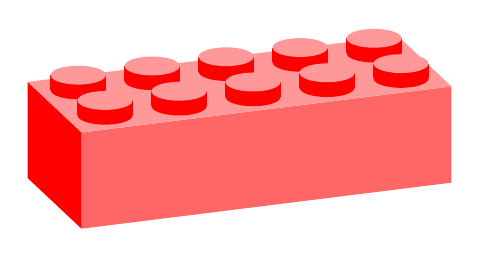
\begin{tikzpicture}
    \brick{5}{2}
  \end{tikzpicture}
}: The smalles brick that doesn't exist yet. Similarly to Lego™, in software, there are building blocks that fit together with pre-made studs and holes. This "connection" between different programs is commonly referred to as an API (Application Programming Interface). Contrary to Lego™, where all bricks have the same studs and holes, the API for most programs is different. To solve this, an API can follow a \textit{specification}. When two programs follow the same API specification, one can be used as a drop-in replacement for the other, such as replacing SQLite with PostGreSQL, since they both work with SQL.

Similarly to Lego™, programs exist in multiple sizes and serve different purposes. Think of an all-in-one off-the-shelf solution such as NextCloud as a bigger block 
\resizebox{!}{1em}{
  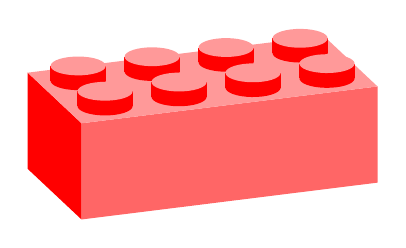
\begin{tikzpicture}
    \brick{4}{2}
  \end{tikzpicture}
}
. It is also possible to get the same functionality by assembling smaller components (blocks), but this is more work
\resizebox{!}{1em}{
  \begin{wall}
    \wallbrick[color=gray]{5}{2}
    \newrow
    \wallbrick[color=red]{1}{2}
    \wallbrick[color=orange]{1}{2}
    \wallbrick[color=yellow]{1}{2}
    \wallbrick[color=green]{1}{2}
  \end{wall}
}
. Specifically, if more than one component is used that requires user authentication, an additional user-authentication block is needed as a base plate that all components need to connect to
\resizebox{!}{1em}{
  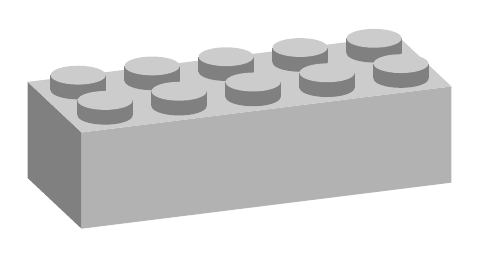
\begin{tikzpicture}
    \brick[color=gray]{5}{2}
  \end{tikzpicture}
}
.
Conversely, once a bigger block is in place, it may be more work to add to it what is actually required (compare 
\resizebox{!}{1em}{
  \begin{wall}
    \addtocounter{brickx}{3}
    \wallbrick[color=gray]{2}{2}
    \newrow
    \wallbrick[color=red]{4}{2}
    \wallbrick[color=blue]{1}{2}
    \newrow
    \addtocounter{brickx}{3}
    \wallbrick[color=orange]{2}{2}
  \end{wall}
} with \resizebox{!}{1em}{
  \begin{wall}
    \wallbrick[color=gray]{5}{2}
    \newrow
    \wallbrick[color=red]{1}{2}
    \wallbrick[color=orange]{1}{2}
    \wallbrick[color=yellow]{1}{2}
    \wallbrick[color=green]{1}{2}
    \wallbrick[color=blue]{1}{2}
  \end{wall}
}).

Finally, it is possible to modify bricks or create new bricks. Contrary to Lego™, good software components themselves are made up of smaller bricks. Thus, if a component needs to be changed, one can look deeper into the brick and extend it. This does cost extra work, since one has to learn the internals of a component, which may be written in an unfamilliar programming language. Alternatively, bigger components often allow for plugin development. This means that one does not need to dive as deeply into the source code to be able to add features.
In this section, both all-in-one solutions and smaller components (microservices) per subject will be discussed. 

\subsubsection{Harmonization, indexing and data storage}

Before we dive into encryption, it is important to understand and evaluate different options for data storage, because that will influence the options for encryption. Storage also affects options for harmonization and indexing (searching) of data, so that will also be discussed here. Geospatial data comes in two categories:

\begin{LaTeXdescription}
  \descitem{Vector data}{data_vector} High-quality, often human-made data such as in-situ soil measurements. These are often (partially) sensitive. Vector data often comes with many different measurements for a single point and is tabular in nature.
  \descitem{Raster data}{data_raster} data from sattelite imagery. This data is often not as sensitive and generally consumes a lot of disk space.
\end{LaTeXdescription}

The data we wish to encrypt is \descref{data_vector}, which is tabular in nature. Tabular data is prolific in many fields of science, where the problem of harmonization and indexing has been addressed. Especially in Biology, the Global Biodiversity Information Facility (GBIF) has made big steps towards harmonizing user-provided data by developing an Integrated Publishing Toolkit (IPT)\cite{robertsonGBIFIntegratedPublishing2014,zizkaNoOnesizefitsallSolution2020}. In this toolkit, data is described by files either using the Darwin Core Specification or Ecological Metadata Language \cite{fegrausMaximizingValueEcological2005}. They also provide a validator that blocks a data provider from uploading their data if they do not adhere to the specification.

For harmonization and indexing, an approach similar to the IPT was taken, but the more field-relevant STAC specification was chosen over the Darwin Core or EML \cite{zhaoScalableSystemSearching2021}. This resolved the question for indexing and metadata. The next question: "How to store the data" is considered next, along with complexities that come with them.

In a general, simplistic view, there are three ways of storing tabular data:

\begin{LaTeXdescription}
  \descitem{Relational database}{storage_rdb} Data is stored in tables in a SQL database such as PostGreSQL, MariaDB, MySQL or SQlite.
  \descitem{Semi-structured database}{storage_mongo} Data is stored in a database, but not necessarily in tables. An example is \href{https://youtu.be/b2F-DItXtZs}{MongoDB}.
  \descitem{Object storage}{storage_object} Data is stored as "files" inside a "file system". Examples include directly storing it on the server file system, Minio and SeaweedFS (S3-compatible storage solutions).
\end{LaTeXdescription}

There are benefits and drawbacks to each of these solutions. They will be shortly discussed, after which the additional component of encryption will be added.

Storing data in a \descref{storage_rdb} requires that all data types in a table are the same. For example: Alice uploads biodiversity data with a \textit{Species} column that has \textit{String} datatype. Bob later wants to also upload biodiversity data, but their \textit{Species} column has \textit{number} datatype. If the database tries to put these two datasets in the same table, it will complain that Bob's data cannot be put in this table. For harmonization purposes, this is highly desireable, since both Alice and Bob have to upload their data in the same dataformat. For the server design, however, this introduces a maintenace load on the server administrator/design, since tables have to be made for every dataset or type of data that is stored. Adding new data to an existing table, as well as access to data by many users is very fast using this database type.

MongoDB, the only considered \descref{storage_mongo} stores its data as JSON objects. This is highly beneficial if the data is already in JSON format, such as with STAC data. However, if data is not in this format, it needs to be converted (serialized). Additionally, adherence to a schema is not enforced by design, but has to be implemented at another architectural layer. Appending data to an existing document, as well as querying is also very fast in MongoDB.

\descref{storage_object} is the most flexible storage type. It allows for any file to be stored and quickly accessed, regardless of whether it is even tabular data. Harmonization, indexing and appending data are all ofloaded to higher architectural layers. This does not mean that appending data in Object storage cannot be fast, but that it depends on the file type under which it is stored. Popular tabular file types for geospatial data include CSV, MBTiles, \href{http://www.geopackage.org/spec/}{GeoPackage} and \href{https://geoparquet.org/}{Apache Parquet}. CSV is the simplest data format, which can be easily edited by hand or reasoned about. MBTiles and GeoPackage are both an SQLite database with additional specification. Thus, any operation that can be applied to an \descref{storage_rdb}, such as appending rows, can also be applied to a GeoPackage or MBTiles dataset. However, when manually editing such data through SQL, care should be taken to adhere to the specification. Apache Parquet is another data format that uses Apache Arrow for fast data access and manipulation.

% Upon inspecting the IPT source code, it was found that data is stored in a customizable data directory on the server, which is indeed (\descref{storage_object}). EteSync, an end-to-end encryption solution stores encrypted 

This far, no conclusion about which storage service could be used can be drawn. They do differ in their level of encryption support, which is discussed next.

\subsubsection{\texorpdfstring{\includesvg[height=1em]{../principles/FAIR/accessible/protocol_icon.svg}}{} Encryption-in transit}

\includesvg[height=1em]{../principles/FAIR/accessible/protocol_icon.svg} Encryption-in-transit is a well-established terrain and solve-all off-the-shelf solutions are available (\descref{https_cryptbot} and \descref{https_caddy}).
Put very simply, all data transfer we are planning to do is done over HTTP (HyperText Transfer Protocol). \href{https://en.wikipedia.org/wiki/HTTPS}{HTTPS} (HTTP + Secure) provides encryption-in-transit for this protocol.
HTTPS has been around since 1996 and has noticeably evolved, fixing major security flaws in the first few iterations. Therefore, the web server should be configured to use the most up-to-date version of encryption possible. Specifically, TLS1.3 (Transport Layer Security) is needed, which should also be used for the internal network in the case of sensitive data. Below is a short summary of tools used for encryption-in-transit.

\begin{LaTeXdescription}
  \descitem{self-signed TLS}{https_selfsign} Encryption-in-transit where the admin signs their own certificates. This is useful for internal communication. If used on client-facing pages, most browsers will issue a warning.
  \descitem{cryptbot}{https_cryptbot} command-line utility for managing https with any well-known server software.
  \descitem{Caddy}{https_caddy} Server software that automatically issues certificates with minimal necessary configuration. Typically used as a reverse proxy.
\end{LaTeXdescription}

Regardless of which encryption scheme is further used, encryption-in-transit should still be used. This is a de-facto standard and is easy enough to set up.

\subsubsection{Encryption and key management}

In the layout diagrams, \includesvg[height=1em]{../principles/GDPR/encryption.svg} encryption has been denoted by the padlock symbol. The encryption scheme to use (the padlock itself) is the easy part of the problem. Solid, battle-tested encryption schemes exist - that is: there are enough "unbreakable" padlocks to choose from. The harder part is \includesvg[height=1em]{../icons/key-solid.svg}key management, because this is application-specific. The same problems that apply to managing house keys also apply to managing cryptographic keys:
\begin{enumerate}
  \item If you give someone a key, they will always be able to open the lock, unless the lock is changed.
  \item If all keys are lost, the data is lost ("unbreakable" padlocks).
  \item If a key could have been stolen, all locks need to be changed.
\end{enumerate}
It should be noted here, that in the computer world compared to the real world: There are much more keys, much more users, much more sharing, much more stealing and is is much easier to be sloppy, especially for less technically inclined people. Because of this, most applications do the key management for the user. Additionally, special Key Management Services (KMS) exist that handle keys separately from the application. Using a KMS alongside other applications that manage keys poses a \resizebox{!}{1em}{
  \begin{wall}
    \addtocounter{brickx}{3}
    \wallbrick[color=gray]{2}{2}
    \newrow
    \wallbrick[color=red]{4}{2}
    \wallbrick[color=blue]{1}{2}
    \newrow
    \addtocounter{brickx}{3}
    \wallbrick[color=orange]{2}{2}
  \end{wall}
}-problem: The user now needs to authenticate to both the KMS and other application, and access to data and keys should be kept in sync between both the KMS and storage application. An overview of different KMSs is given by \cite{kuzminykhComparativeAnalysisCryptographic2020}.


\subsubsection{End-to-end Encryption}
The pathway into end-to-end encryption was further explored. End-to-end encryption is an established terrain for messaging services like Whatsapp/Signal/Telegram and E-mail (ProtonMail PGP). These are not data repositories, however. Allowing for both public and private data to co-exist, as well as the ability to further share data without re-encrypting it, are parts that have to be developed.

Based on \href{https://github.com/openpgpjs/openpgpjs/discussions/1604#discussioncomment-5099620}{this answer} on a discussion I created, two different implementations using PGP end-to-end encryption were considered, named \textit{Quick PGP} and \textit{Hacky PGP}. \textit{Quick PGP} would require additional database management to separately store all access keys, and \textit{Hacky PGP} would require modifying the PGP-encrypted BLOB according to the OpenPGP specification (\href{https://www.rfc-editor.org/rfc/rfc4880}{RFC 4880}). An overview of different encryption solutions is shown in table \ref{tab_optionsComparison}, which was created in deliverable \ref{del_e2ePresentation}.  After the presentation, Leandro suggested EteSync as an additional solution that works out-of-the box for end-to-end encryption.

Appending data to a table that is end-to-end encrypted introduces difficulties. If an entire column is encrypted together, this reduces the attack surface, but requires the data provider to: 1. download the entire column 2. append the data 3. encrypt the entire column 4. upload the data. If files are large, this requires a lot of extra network usage. Alternatively, a sensitive column could be encrypted separately per row. This has three major drawbacks. Firstly, it increases disk usage, since encryption requires data to be aligned to blocks that are larger than what is normally in a single table cell. Secondly, it increases the attack surface if all values are encrypted with the same key. Thirdly, it requires a bit more computation. One data format that has struck a balance between these extremes is Parquet Modular Encryption. In Parquet Modular Encryption, data is encrypted per "page", which includes several rows. Additionally, it uses a scheme with multiple keys that are encrypted by one user-provided "Master" key. This allows changing the user-provided key with less effort, increasing security.

\begin{table}[!t]
  \renewcommand{\arraystretch}{1.3}
  \caption{Comparison of End-to-end encryption options}
  \centering
  % https://stackoverflow.com/a/50251364
  \resizebox{\linewidth}{!}{
  \begin{tabular}{l|c|c|c|c|c|c|}
  \hline
  & Implement & Upload & Decrypt & YubiKey? & "Niceness" & Standards \\
  \hline
  Quick PGP & \cellcolor[named]{ForestGreen}++ & \cellcolor[named]{BrickRed}- - & \cellcolor[named]{ForestGreen}+ & \cellcolor[named]{ForestGreen}$✓$ & \cellcolor[named]{BrickRed}- - & \cellcolor[named]{ForestGreen}++ \\
  Hacky PGP & \cellcolor[named]{BrickRed}- & \cellcolor[named]{ForestGreen}+ & \cellcolor[named]{ForestGreen}+ & \cellcolor[named]{ForestGreen}$✓$ & \cellcolor[named]{ForestGreen}+ & \cellcolor[named]{ForestGreen}++ \\
  SaltPack & \cellcolor[named]{BrickRed}- - & \cellcolor[named]{ForestGreen}+ & \cellcolor[named]{BrickRed}- - & \cellcolor[named]{BrickRed}$\times$ & \cellcolor[named]{ForestGreen}+ & \cellcolor[named]{BrickRed}- \\
  NextCloud & \cellcolor[named]{BrickRed}- - & \cellcolor[named]{ForestGreen}+ & ? & \cellcolor[named]{BrickRed}$\times$ & \cellcolor[named]{ForestGreen}++ & ? \\
  \hline
  EteSync & \cellcolor[named]{BrickRed}- & \cellcolor[named]{ForestGreen} + & \cellcolor[named]{ForestGreen}+ & \cellcolor[named]{BrickRed}$\times$ & \cellcolor[named]{ForestGreen} & ?\\
  \hline
  \end{tabular}}
  \label{tab_optionsComparison}
\end{table}

\subsubsection{\texorpdfstring{\includesvg[height=1em]{../principles/GDPR/protection_rest.svg}}{} Encryption-at-rest}
Encryption-at-rest is a more intricate terrain than encryption-in-transit. With encryption-in-transit, only two parties - the sending and receiving party - should be able to decrypt the data (authorization). Furthermore, authentication is an established terrain in encryption-in-transit using TLS certificates. With encryption-at-rest, however, there are a variable number of parties that should be able to decrypt the data: The data provider and anyone the data is shared with (authorization). Furthermore, authentication and is handled by the application ("Logging in") - which works differently for many applications. Additionally, the keys for decrypting the data should be securely stored and shared with only authenticated and authorized users. 

A variety of solutions were considered, which had differing levels of production-readiness. These can be split into \descref{ear_object}, \descref{ear_database} and \descref{ear_e2e}. \descref{ear_object} refers to a system where data is stored as files, as opposed to \descref{ear_database}, where data is stored in a database as records in tables.

\begin{LaTeXdescription}
  \descitem{Object-level encryption}{ear_object} Full-file encryption provided by the object storage
  \begin{LaTeXdescription}
    \descitem{S3}{ear:obj_s3} 
  \end{LaTeXdescription}
  \descitem{In-file encryption}{ear_infile} partial file encryption for specific formats.
  \begin{LaTeXdescription}
    \descitem{Parquet Modular Encryption}{ear_infile_parquet} for (geo)parquet files. Allows per-column encryption.
    \descitem{SQlite (SQLCipher)}{ear_db_sqlite} Open source version only allows full-table encryption.
  \end{LaTeXdescription}
  \descitem{Database encryption}{ear_database} Relational database encryption at database level. Most databases allow per-value encryption, since databases are often used to store passwords that could be additionally encrypted per-user.
  \begin{LaTeXdescription}
    % \descitem{PostGreSQL}{ear_db_postgres} \href{https://stackoverflow.com/a/61200974/14681457}{SE}, Full-database: TDE, per-column: pg_grypto.
    \descitem{MariaDB}{ear_db_mariadb} Per-table encryption and Key Management Plugins.
    \descitem{MySQL}{ear_db_mysql} Per-table\textit{space} encryption
    \descitem{MongoDB}{ear_obj_mongo} via MongoDB Queryable Encryption
  \end{LaTeXdescription}
  \descitem{Key Management Service (KMS)}{ear_kms} Adapted from \cite{kuzminykhComparativeAnalysisCryptographic2020}, table 4.
  \begin{LaTeXdescription}
    \descitem{CyberArk Conjur}{ear_kms_conjur}
    \descitem{HashiCorp Vault}{ear_kms_vault}
    \descitem{OpenStack Barbican}{ear_kms_barbican}
    \descitem{Pinterest Knox}{ear_kms_knox}
    \descitem{Square KeyWhiz}{ear_kms_keywhiz}
  \end{LaTeXdescription}
  \descitem{End-to-end encryption}{ear_e2e} 
  \begin{LaTeXdescription}
    \descitem{Etesync}{ear_e2e_ete}
    \descitem{Cryptdrive}{ear_e2e_cryptdrive}
    \descitem{DIY PGP}{ear_e2e_pgp}
    \descitem{DIY TweetNaCl}{ear_e2e_nacl}
    % \descitem{MongoDB Explicit Client-Side Field Level Encryption}{ear_e2e_mongo}
  \end{LaTeXdescription}
\end{LaTeXdescription}

\subsubsection{Templating and signing}
The following document management and signing softwares were found that claimed to be open source:
\begin{LaTeXdescription}
  \item[all-in-one:] Both Document management and Document signing
  \begin{enumerate}
    \item PandaDoc
    \item Odoo
  \end{enumerate}
  \item[Document signing:] Digital signing for PDF documents
  \begin{enumerate}
    \item DocuSign
    \item LibreSign (Nextcloud)\label{sign_LibreSign}
  \end{enumerate}
  \item[Low-level digital signing:] SignServer
\end{LaTeXdescription}
DocuSign does not claim to be open source, but was the signing solution that is currently in use at OGH.
However, only Libresign (\ref{sign_LibreSign}) was fully open source, other signing softwares only open sourced their API, while running the signing and document management as Software as a Service (SaaS). I did give a presentation, but did not create an extensive overview of different levels of electronic signatures, even though I did research that. LibreSign is an Advanced Electronic Signature, as explained by the lead developer \href{https://github.com/LibreSign/libresign/issues/1788#issuecomment-1638228780}{on GitHub}.

\section{Implementation}\label{sec_implementation}

\subsection{Deliverables}

\begin{enumerate}
  \item \href{https://gitlab.opengeohub.org/fee.gevaert/principle-layouts/-/tree/vue}{Principle-layouts icons as a Vue package}
  \item Exploration of using Parquet Modular Encryption \href{https://gitlab.opengeohub.org/fee.gevaert/geoencrypt-vue}{Repository}
  \item \href{https://gitlab.opengeohub.org/fee.gevaert/ogh-gitlab-runner-howto}{Gitlab Runner CI/CD}
  \item \href{https://gitlab.opengeohub.org/fee.gevaert/geoencrypt-docker/-/tree/local}{Nextcloud Docker Compose setup}\label{del_ncDocker}
  \item \href{https://gitlab.opengeohub.org/fee.gevaert/geoencrypt/}{Nextcloud plugin}
  \item GPU-accelerated Seasonal-Trend decomposition: \href{https://gitlab.opengeohub.org/fee.gevaert/hastl}{HaSTL}
\end{enumerate}

% // ⁵√2³=2^(3⁄5)
% // lim x→x₀ f(x) = L ⇔ ∀ε∃δ: |x-x₀|<δ => |f(x)-L|<ε

\subsection{summary}

The transition from analysis/propose to design/implement was not entirely clear-cut. In the previous section, it was decided to use Nextcloud, because it provided the only open source contract signing solution. I gave another presentation with the mockup shown in figure \ref{fig_sharingMockup}, which shows LibreSign as a signing software. Also, OGH uses Google Workspace as a drive and office solution, and wanted to move to Nextcloud. As such, I was given the task of setting up a Nextcloud. This was a long, arduous task, since there are many different configurations to use nextcloud, which I've documented in deliverable \ref{del_ncDocker}. There, I have provided instructions for setting up Nextcloud in the following configurations:

\begin{LaTeXdescription}
  \descitem{Snap}{nc_snap}: Install Nextcloud directly through snap. No additional plugins possible
  \descitem{Bare-metal}{nc_bare}: Install and configure Nextcloud manually through the default system package manager. This requires a lot of configuration and maintenance and is not reproducible.
  \descitem{All-In-One}{nc_aio}: Install using the convenience All-In-One docker deployment. This cannot use S3 as a primary storage and thus cannot provide encryption-at-rest.
  \descitem{Custom Docker Compose}{nc_docker}: Install using custom Docker build and/or compose files.
\end{LaTeXdescription}

All configurations I tested locally and if they needed DNS resolution, on my personal server \href{https://wur.pm}{wur.pm}. 
\descref{nc_snap} does not allow to install \textit{any} additional plugins and also gives \textit{no} control over which database backend is used. For our use-case, this was unacceptable.
\descref{nc_bare} was a good exercise for me to understand the deployment and workings of Nextcloud, but is too much work to set up and maintain for serious production deployment.
\descref{nc_aio} Is a really nice way of deploying Nextcloud. However, since there is \href{https://github.com/nextcloud/all-in-one/discussions/1807}{no support} for S3 as a primary storage, there is no support for server-side encryption, which is a prerequisite in the GDPR for handling sensitive data.
\descref{nc_docker} was the only logical option left to deploy Nextcloud. \href{https://www.docker.com/}{Docker} is a containerization and orchestration platform. In Lego™-speak: Docker is the tool that assembles the Lego™ bricks. Let's say we have a web application with a database(\resizebox{!}{1em}{
  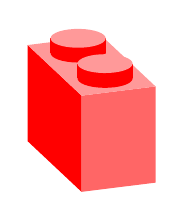
\begin{tikzpicture}
    \brick[color=red]{1}{2}
  \end{tikzpicture}
}), back-end code (\resizebox{!}{1em}{
  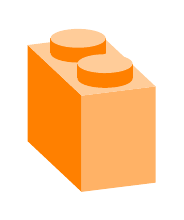
\begin{tikzpicture}
    \brick[color=orange]{1}{2}
  \end{tikzpicture}
}) and front-end code (\resizebox{!}{1em}{
  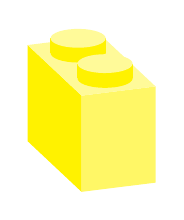
\begin{tikzpicture}
    \brick[color=yellow]{1}{2}
  \end{tikzpicture}
}), then a full application is started with Docker: \resizebox{!}{1em}{\begin{wall}
  \wallbrick[color=red]{1}{2}
  \wallbrick[color=orange]{1}{2}
  \wallbrick[color=yellow]{1}{2}
\end{wall}}.

% as explained below:
% \blockquote{Software containers are lightweight computational environments containing all necessary elements (code, dependencies, data, configuration, etc.) to execute a certain process [62]. For example, a software container used for research can be a simple Linux environment containing only a specific Python version installed together with analysis packages such as Tensorflow [63].}
That means that it runs applications inside "containers", which are a full operating system (OS) like a virtual machine, but more lightweight and slightly less secure. Since containers provide a full operating system, they are independent of the host OS and thus provide a fully reproducible environment: In stead of installing - for example - PostGreSQL on an operating system that may have another database running or conflicting dependencies, an image containing a fully configured installation of PostGreSQL is downloaded and started. To then run Nextcloud with PostGreSQL as a database, Docker-compose is used.

Using docker-compose, so-called \textit{compose files} can be created that specify which containers should be started with which configuration and on which ports they should communicate with each other. Like this, sharing a compose file is a completely reproducible way to deploy a system. I created compose files for Nextcloud (full deployment), Minio (S3 primary storage) and Caddy (reverse proxy) that could be separately started. This was especially useful because I could just start Nextcloud without Caddy for development purposes. Also Leandro used Apache as a reverse proxy and SeaweedFS as an S3 backend, both of which are more verbose to set up than Caddy or Minio. Using this setup, I could test the deployment, while being easily transferable to the actual OGH systems.

Now the development and deployment setups were in place, it was time to start developing the plugin. Initially, Leandro told me to use parquet files, which I epxlored reading and splitting on the client-side. I created a short overview of technical possibilities \href{https://docs.google.com/document/d/1R5wIZc0mxVcqyIUatDX1DlvIh9arl41VQ3EWcYc8NQE/edit?usp=sharing}{in my notes}.
However, the parquet file format does not have an index column, nor a default JOIN operation, as was clarified to me in \href{https://github.com/apache/arrow/issues/31458#issuecomment-1494961959}{This github issue}. Parquet \textit{does} offer Parquet Modular Encryption, which allows to separately encrypt the columns of a parquet file. Parquet Modular encryption leverages the data structure of a parquet file to make it very space- and time-efficient. However, the only interface provided to access and decrypt keys, is through defining an interface to a Key Management service (KMS) client. I think it would have been possible to manage keys using EteSync or Nextcloud as a rudimental KMS, but ChatGPT strongly encouraged me to use a dedicated KMS. Within this specific issue, there was also no person within OGH to ask for support, so I took ChatGPT's advice.

After I gave the architectures presentation \ref{del_architectures} and talked with Leandro, it was decided that I would create an easy Nextcloud plugin that would process CSV files in the initial phase.

\subsubsection{Nextcloud plugin development}

The rest of my internship, I spent on developing the Nextcloud plugin to split a CSV into multiple files. This is a simplified version of the interactions as shown in figure \ref{fig_sequenceDiagram}, with a visual mockup, shown in \ref{fig_sharingMockup}, as shared with OGH in \ref{del_e2ePresentation}.

\begin{figure}
  \centering
  \includegraphics[width=1\linewidth]{img/InterfaceMockup.png}
  \caption{Mockup of the Minimum Valuable Product}
  \label{fig_sharingMockup}
\end{figure}

Documentation for plugin development in Nextcloud was limited and dependency management development in Javascript is a big hassle.
Specifically, Vue is transitioning from 2.7 to 3, with planned End-Of-Life for Vue 2 in 31 December 2023, after which Vue 2 will no longer receive security updates.
Since we are designing a high-security plugin, it is paramount to make this transition.
Most Nextcloud provided packages -that deliver essential functionality for easily developing a plugin-, however, require Vue 2.7. Therefore, I had to develop the plugin in Vue 2.7 to be able to use those packages.
Luckily, Vue 2.7 offers the Vue 3 API \textit{as well as} the Vue 2 API. Thus, the plugin can be written in Vue 2.7 in such a way that no code needs to be rewritten to change to Vue 3. Dependency management, however, still needs to be done to go through the transition. This means that all used Nextcloud packages need to have their Vue 3 version available.

Because the documentation was limited, I mostly resorted to reading source code of Nextcloud plugins that had implemented similar functionality. This was, however not as effective as I had hoped, since most plugins I found were written in Vue 2.

Additionally, the Vue build system changed to Vite, and the Nextcloud plugin scaffold uses a different build system. The only plugin that uses Vite+Typescript as a build system I found was \href{https://github.com/nextcloud/logreader}{logreader}.

Because the idea was still to maybe transition to something else than NextCloud, the use of back-end code was kept to a minimum. I did not find a package that aids the creation of STAC entries, only packages that verify whether a JSON datastructure adheres to the STAC specification.

Through all these hurdles, the plugin was developed. Firstly, it allows users to split a CSV into sensitive columns and uploads them to a folder whose name is deterministically determined from the filename. Then, the remaining public columns are put in a \textit{"public"} folder together with the STAC entries, which is retrievable through a link share.

The second part - templating and contract signing - was only partially developed. This far, everything had been developed on the front-end, but for linking a file to a contract, back-end code was needed. This meant that I had to learn PHP, which took more time. The database schema used for linking a contract is shown in figure \ref{fig_dbSchema}. It should be noted, that contracts in LibreSign are public by default, see the \href{https://github.com/LibreSign/libresign/issues/686}{Github Issue}. 

\begin{figure}
  \centering
  \includegraphics[width=.75\linewidth]{img/dbSchema.png}
  \caption{Database schema for the Nextcloud implementation}
  \label{fig_dbSchema}
\end{figure}

This concluded the plugin development thus far. This implementation is a \resizebox{!}{1em}{
  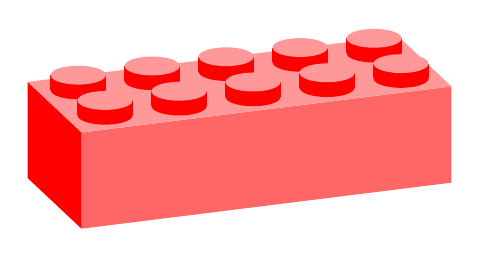
\begin{tikzpicture}
    \brick{5}{2}
  \end{tikzpicture}
}-style implementation: The plugin uses Nextcloud-provided packages and its API. Effort has been made to make the extension (\resizebox{!}{1em}{
  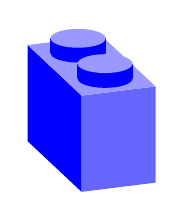
\begin{tikzpicture}
    \brick[color=blue]{1}{2}
  \end{tikzpicture}
}) easily separable from Nextcloud (\resizebox{!}{1em}{
  \begin{wall}
    \wallbrick{4}{2}
    \wallbrick[color=blue]{1}{2}
  \end{wall}
}), so it can be implemented in e.g. EteSync (\resizebox{!}{1em}{
  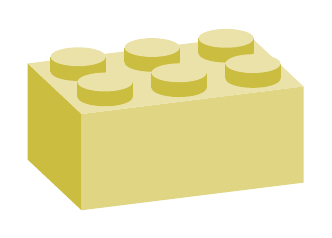
\begin{tikzpicture}
    \brick[color=yellow!80!blue]{3}{2}
  \end{tikzpicture}
}), where it will also use EteSync's API (\resizebox{!}{1em}{
  \begin{wall}
    \wallbrick[color=yellow!80!blue]{4}{2}
  \end{wall}
}).

\subsubsection{Side project: HaSTL}

Besides the internship assignment, I also set up a Docker environment for running a GPU-accelerated Seasonal trend decomposition that was much faster than the equivalent implementation from SciPy. It was a fun endeavour, for which I derived the following workflow:
\begin{enumerate}
  \item Install drivers
  % \item Try to run \href{https://github.com/not-an-aardvark/lucky-commit}{lucky_commit} on the GPU
  \item Try to run HaSTL on the GPU
  \item repeat steps 1-3 inside docker
\end{enumerate}
Installing and running HaSTL, together with speed comparisons concluded this side project.
\section{Discussion}


Because I first made the principles, and started developing a sharing app later, I wanted the proof-of-concept to adhere to all the principles. Therefore, the focus was directly on a public/private sharing system with multiple users, where access can be given or revoked. This is a much more complex scenario than sending files encrypted to a single, trusted person who can only decrypt it with a hardware key - that can be directly done with PGP. This would have made a different proof-of-concept, with the risk of lock-in: Allowing for revoking access and sharing after encryption is a non-trivial task in PGP.


Additionally, software architecture design tools and the principle icons could be further integrated. They were used in the plugin UI to foster adoption of the principles. Since these icons are unambiguously linked to the principles, they can be used as a checklist for which principles are implemented in a software. Designing computer architecture, however, does not have a single workflow due to the variety of different computer systems. This makes enahncing a workflow for incorporating these diagrams -and with them the principles- difficult. This may inhibit further adoption of the principles or inter-displinary communication about computer architecture.

No user-testing was done. This applies to both the principles overview, as well as the developed plugin. Thus, even though the ideas are there and the proof-of-concept implementations are there, it remains a fully open question whether they will be adopted.

\section{Conclusion}

The internship is done, the report should be a pointer for further work.

% use section* for acknowledgment
\section*{Acknowledgment}

I would like to thank all the people at OGH who have supported me during my internship and have created a healthy work environment where brain-bumping smoothly coincides with serious work and personal conversation. Special thanks go to Ichsani - my host supervisor, who didn't always have the technical knowledge needed to assist me, but gave the emotional support, structure and lenience when needed so that I could work, learn and grow into the inspiring environment that is OGH.
Honourable mentions go to Murat - my front-end office mate, Leandro and YuFong - go-to supernerds for DevOps questions and Rolf - my later office mate who just knew everything and was very chill in sharing his wealth.
I'm really tired now and want to hand in my report. To people that were important but are not in here, that is the reason. Please know you are also appreciated. Here's a duck to show it:
  
\begin{tikzpicture}
    \duck[xshift=100,scale=1,lightsaber=yellow,graduate=gray!20!black,
    tassel=red!70!black]
  \end{tikzpicture}
.

\ifCLASSOPTIONcaptionsoff
  \newpage
\fi


\printbibliography
\end{document}


